%intestazione tipo degli appunti di matematica

\documentclass[a4paper, oneside]{article}
\usepackage[utf8]{inputenc}
\usepackage{graphicx}
\usepackage{caption}
	\captionsetup{format=hang,labelfont={sf,bf}}
\usepackage{multicol}
\usepackage{ulem}
\usepackage{lipsum} 
\usepackage[leqno,intlimits]{amsmath}
\usepackage{amssymb}
\usepackage{amsthm}
\usepackage{yhmath}
\usepackage[leqno,fleqn,intlimits]{empheq}
\usepackage{pgfplots}
	\pgfplotsset{/pgf/number format/use comma,compat=newest}
\usepackage{xcolor}
\usepackage{framed}
\usepackage{cancel}
\usepackage[colorlinks]{hyperref}
	\hypersetup{
	     colorlinks=true,
	     linkcolor=blue,
	     filecolor=blue,
	     citecolor = black,      
	     urlcolor=cyan,
	     }
\usepackage{ifthen}
\usepackage{intcalc}
\usepackage[most]{tcolorbox}
\usepackage{forest}
\usepackage{booktabs}

%%%%%%%%%%%%%%%%%%%%%%%%%%%%%%%%%%%%%%%%%%%%%%%%%%%%%%%%%%%%%%%%%%%%%%%%%%%%%%%%%%%%%%%%%%

	% Comandi per la creazione del riquadro attorno alle equazioni
	\newif\ifmarg
	\margtrue
	\ifmarg
	\makeatletter
	\let\mytagform@=\tagform@
	\def\tagform@#1{\maketag@@@{\mbox{~}\hbox{\rlap{\hspace{0.5in}(\ignorespaces#1\unskip\@@italiccorr)}}}\kern1sp}
	\renewcommand{\eqref}[1]{{\mytagform@{\ref{#1}}}}
	\makeatother
	\fi
	
	\newcommand*\mygraybox[0]{%
		\tcbhighmath}
		
	\newcommand{\equazione}[1]{	\begin{empheq}[box=\mygraybox]{equation*}
			#1
		\end{empheq}}
	%%%%%%%%%%%%%%%%%%%%%%%%%%%%%%%%%%%%%%%%%%%%%%%%%%%%%%%%%%%%%%%%%%%
	% Creazione dell'ambiente ``NOTA'' 
		\newlength\sidebar
		\newlength\envrule
		\newlength\envborder
		\setlength\sidebar{1.5mm}
		\setlength\envrule{0.4pt}
		\setlength\envborder{2.5mm}
		
		\makeatletter
		\long\def\fboxs#1{%
		  \leavevmode
		  \setbox\@tempboxa\hbox{%
		    \color@begingroup
		      \kern\fboxsep{#1}\kern\fboxsep
		    \color@endgroup}%
		  \@frames@x\relax}
		\def\frameboxs{%
		  \@ifnextchar(%)
		    \@framepicbox{\@ifnextchar[\@frameboxs\fboxs}}
		\def\@frameboxs[#1]{%
		  \@ifnextchar[%]
		    {\@iframeboxs[#1]}%
		    {\@iframeboxs[#1][c]}}
		\long\def\@iframeboxs[#1][#2]#3{%
		  \leavevmode
		  \@begin@tempboxa\hbox{#3}%
		    \setlength\@tempdima{#1}%
		    \setbox\@tempboxa\hb@xt@\@tempdima
		         {\kern\fboxsep\csname bm@#2\endcsname\kern\fboxsep}%
		    \@frames@x{\kern-\fboxrule}%
		  \@end@tempboxa}
		\def\@frames@x#1{%
		  \@tempdima\fboxrule
		  \advance\@tempdima\fboxsep
		  \advance\@tempdima\dp\@tempboxa
		  \hbox{%
		    \lower\@tempdima\hbox{%
		      \vbox{%
		        %\hrule\@height\fboxrule
		        \hbox{%
		         \vrule\@width\fboxrule
		          #1%
		          \vbox{%
		            \vskip\fboxsep
		            \box\@tempboxa
		            \vskip\fboxsep}%
		          #1%
		          }%\vrule\@width\fboxrule}%
		        }%\hrule\@height\fboxrule}%
		                          }%
		        }%
		}
		\def\esefcolorbox#1#{\esecolor@fbox{#1}}
		\def\esecolor@fbox#1#2#3{%
		  \color@b@x{\fboxsep\z@\color#1{#2}\fboxs}{\color#1{#3}}}
		\makeatother
		
		\definecolor{exampleborder}{rgb}{0.5, 0.5, 0.5}
		\definecolor{examplebg}{rgb}{0.89, 0.89, 0.89}
		\definecolor{statementborder}{rgb}{.9,0,0}
		\definecolor{statementbg}{rgb}{1,.9,.9}
		
		\newenvironment{eseframed}{%
		  \def\FrameCommand{\fboxrule=\the\sidebar  \fboxsep=\the\envborder%
		  \esefcolorbox{exampleborder}{examplebg}}%
		  \MakeFramed{\FrameRestore}}%
		 {\endMakeFramed}
		
		\newenvironment{nota}[1]
		{\par\medskip%\refstepcounter{esempio}%
		\hbox{%
		\fboxsep=\the\sidebar\hspace{-\envborder}\hspace{-.5\sidebar}%
		\colorbox{exampleborder}{%
		\hspace{\envborder}\footnotesize\sffamily\bfseries%
		\textcolor{white}{{{\large
		#1}}\hspace{\envborder}}
		}
		}
		\nointerlineskip\vspace{-\topsep}%
		\begin{eseframed}\noindent\ignorespaces%
		}
		{\end{eseframed}\vspace{-\baselineskip}\medskip}
	%%%%%%%%%%%%%%%%%%%%%%%%%%%%%%%%%%%%%%%%%%%%%%%%%%%%%%%
	\newcounter{tartaglia}
	\newcounter{newton}
	\newcounter{i}% contatore delle righe
	\newcounter{j}% contatore delle colonne
	\newcounter{n}% è il numero massimo di righe
	\newcounter{I}% contatori di servizio
	\newcounter{J}%
	
	%creazione del comando ``cbinomiale''
	\newcommand{\cbinomiale}[2]{%
		\intcalcDiv{\intcalcFac{#1}}{\intcalcMul{\intcalcFac{#2}}{\intcalcFac{\intcalcSub{#1}{#2}}}}
	}
	
	%creazione del comando ``Binomio di Newton''
		\newcommand{\newton}[1]{%
			\stepcounter{newton}%
			\setcounter{i}{1}%
			\setcounter{j}{0}%
			\setcounter{n}{#1}%
				\begin{center}
				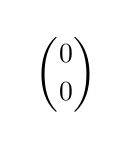
\begin{tikzpicture}[node distance=15 mm]
					\node (\thenewton_n0_0){$\displaystyle\binom{0}{0}$};
					\whiledo{\thei<\then}{%
					\setcounter{I}{\thei}%
					\addtocounter{I}{-1}%
						\whiledo{\thej<\thei}{%
							\setcounter{J}{\thei}%
							\addtocounter{J}{-1}%
								\node[below left of=\thenewton_n\theI_\thej](\thenewton_n\thei_\thej){$\displaystyle\binom{\thei}{\thej}$};
								\stepcounter{j}%
							}
						\node[below right of=\thenewton_n\theI_\theJ](\thenewton_n\thei_\thej){$\displaystyle\binom{\thei}{\thej}$};
						\stepcounter{i}%
						\setcounter{j}{0}%
					}
				\end{tikzpicture}
				\end{center}
	}
		
	%creazione del comando ``Triangolo di Tartaglia''
		\newcommand{\tartaglia}[2]{%
			\stepcounter{tartaglia}%
			\setcounter{i}{1}%
			\setcounter{j}{0}%
			\setcounter{n}{#1}%
				\begin{center}
				\begin{tikzpicture}[node distance=#2 mm]
					\node (\thetartaglia_t0_0){\cbinomiale{0}{0}};
					\whiledo{\thei<\then}{%
					\setcounter{I}{\thei}%
					\addtocounter{I}{-1}%
						\whiledo{\thej<\thei}{%
							\setcounter{J}{\thei}%
							\addtocounter{J}{-1}%
								\node[below left of=\thetartaglia_t\theI_\thej](\thetartaglia_t\thei_\thej){\cbinomiale{\thei}{\thej}};
								\stepcounter{j}%
							}
						\node[below right of=\thetartaglia_t\theI_\theJ](\thetartaglia_t\thei_\thej){\cbinomiale{\thei}{\thej}};
						\stepcounter{i}%
						\setcounter{j}{0}%
					}
				\end{tikzpicture}
				\end{center}
	}

%%%%%%%%%%%%%%%%%%%%%%%%%%%%%%%%%%%%%%%%%%%%%%%%%%%%%%%%%%%%%%%%%%%%%%%%%%%%%%%%%%%%%%%%%%%

%ridefinizione comandi
	\newcommand{\example}{\paragraph{Esempio}}
	\newcommand{\tesi}{\noindent\textit{tesi.}\hspace{1em}}
	\newcommand{\gradi}{$^\text{o}$ }
	\newcommand{\CE}{\text{CE}\hspace{0.5em}}
	\newcommand{\pin}[1]{\frac{\pi}{#1}}
	\newcommand{\modulo}[2]{\Big[#1\Big]_{#2}}
	\newcommand{\pimod}[1]{\Big[#1\Big]_{2\pi}}
	\DeclareMathOperator{\arcsec}{arcsec}
	\DeclareMathOperator{\arccot}{arccot}
	\DeclareMathOperator{\arccsc}{arccsc}
	\newcommand{\R}{\mathbb{R}}
	\newcommand{\mezzo}{\frac{1}{2}}
	\newcommand{\pimezzi}{\frac{\pi}{2}}
	\newcommand{\mm}[1]{$\displaystyle#1$}

%%%%%%%%%%%%%%%%%%%%%%%%%%%%%%%%%%%%%%%%%%%%%%%%%%%%%%%%%%%%%%%%%%%%%%%%%%%%%%%%%%%%%%%%%%%


\title{Esercizio Verifica}
\date{11 gen 2021}
\author{Davide Peccioli}

\begin{document}
 	\maketitle
	
	\begin{nota}{Testo}
	\begin{itemize}
	\item[\textit{i.}] Determinare i parametri $a, b\in\R$ in modo che la curva di equazione $$\displaystyle y=f(x)=\frac{ax^3}{x^2-b}$$ abbia nel punto $P\Big(1; \frac{1}{3}\Big)$ la tangente $r$ perpendicolare alla retta $$t: 18x+22y+99=0$$
	\item[\textit{ii.}] Posto $a=-1$ e $b=4$
		\begin{itemize}
		\item [\textit{a.}] Calcolare la derivata della funzione
		\item[\textit{b.}] Studiare e tracciare il grafico probabile della funzione ottenuta
		\end{itemize}
	\end{itemize}
	\end{nota}
	
	\section*{\textit{i.}}
	
	Il testo impone le seguenti condizioni:
	\begin{itemize}
	\item il punto $P$ appartiene alla curva;
	\item la retta tangente alla curva in $P$ è perpendicolare alla retta $t$.
	\end{itemize}
	Poiché l'equazione generica di una retta tangente alla curva $f(x)$ in un suo punto di ascissa $x=x_0$ è 
	\[
	y-f(x_0)=f'(x_0)(x-x_0)
	\]
	posso scrivere queste condizioni come sistema:
	\begin{equation*}
		\begin{cases}
		\displaystyle\frac{1}{3}=\frac{a\cdot(1)^3}{(1)^2-b}\\
		y-1/3=f'(1)(x-1)\perp 18x+22y+99=0
		\end{cases}
	\end{equation*}
	
	Per risolvere la seconda condizione è necessario iniziare calcolando la derivata prima della funzione.
	\begin{multline*}
		f'(x)=\frac{D[ax^3]\cdot(x^2-b)-(ax^3)\cdot D[x^2-b]}{(x^2-b)^2}=\\
		=\frac{3ax^2(x^2-b)-2ax^4}{(x^2-b)^2}=ax^2\cdot\frac{x^2-3b}{(x^2-b)^2}
	\end{multline*}
	\[
	f'(1)=a\cdot\frac{1-3b}{(1-b)^2}
	\]
	
	Si noti inoltre che affinché le due rette siano perpendicolari, deve essere rispettata questa condizione
	\[
		r\perp t \iff 18\cdot f'(1)-22=0\implies f'(1)=11/9
	\]
	
	Il sistema da risolvere, in definitiva, si riduce a
	\[
	\begin{cases}
		\displaystyle1/3=\frac{a}{1-b}\\
		\displaystyle\frac{a(1-3b)}{(1-b)^2}=11/9
	\end{cases}
	\]
	\[
	\begin{cases}
		3a=1-b\\
		11(1-b)^2=9a(1-3b)
	\end{cases}
	\]
	\[
	\begin{cases}
		a=(1-b)/3\\
		11(1-b)^2=3(1-b)(1-3b)
	\end{cases}
	\]
	\begin{gather*}
	(1-b)[11(1-b)-3(1-3b)]=0\\
	b=1\quad\lor\quad11-11b-3+9b=0\implies b=4
	\end{gather*}

	\equazione{(a,b)\in\{(0; 1); (-1; 4)\}}
	
	\section*{\textit{ii.}}
	\[
	y=-\frac{x^3}{x^2-4}
	\]
	\subsection*{Derivata}
	\begin{multline*}
		y'=\frac{D[-x^3]\cdot(x^2-4)-(-x^3)\cdot D[x^2-4]}{(x^2-4)^2}=\\
		=\frac{(-3x^2)(x^2-4)-(-x^3)(2x)}{(x^2-4)^2}=\frac{-3x^4+12x^2+2x^4}{(x^2-4)^2}=\\
		=\frac{12x^2-x^4}{(x^2-4)^2}
	\end{multline*}
	\equazione{y'=\frac{12x^2-x^4}{(x^2-4)^2}}
	\subsection*{Grafico probabile}
	\paragraph{CE} $\displaystyle	x\in (-\infty;-2)\cup(-2;2)\cup(2;+\infty)$
	\paragraph{Zeri} $\displaystyle f(x)=0\iff x=0$
	\paragraph{Limiti}
	\begin{align*}
		\lim_{x\to \infty} &\Big[-\frac{x^3}{x^2-4}\Big]=\infty\\
		\lim_{x\to -2^-} &\Big[-\frac{x^3}{x^2-4}\Big]=\frac{8}{0^+}=+\infty\\
		\lim_{x\to -2^+} &\Big[-\frac{x^3}{x^2-4}\Big]=\frac{8}{0^-}=-\infty\\
		\lim_{x\to 2^-} &\Big[-\frac{x^3}{x^2-4}\Big]=-\frac{8}{0^-}=+\infty\\
		\lim_{x\to 2^+} &\Big[-\frac{x^3}{x^2-4}\Big]=-\frac{8}{0^+}=-\infty
	\end{align*}
	
	Le rette
	\equazione{x=-2\qquad x=2}
	sono \textbf{asintoti orizzontali completi}
	
	\paragraph{Asintoti obliqui}
	
	Gli asintoti obliqui, nella forma $y=mx+q$, si ricaveranno per mezzo dei seguenti passaggi.	
	\begin{align*}
		m&=\lim_{x\to\infty}\Big[-\frac{x^3}{x^3-4x}\Big]=-1\\
		q&=\lim_{x\to\infty}\Big[\frac{-x^3+x^3-4x}{x^2-4}\Big]=0
	\end{align*}
	
	La seguente retta, quindi, è asintoto obliquo della funzione
	\equazione{y=-x}
	\newpage
	
	\paragraph{Piano}\textcolor{white}{nascosto}
	
	\begin{center}
	\begin{tikzpicture}
	\begin{axis}
	[axis lines=middle,
	xmin=-10,
	xmax=10,
	ymin=-10,
	ymax=10, 
	enlargelimits, 
	width=13cm,
	xlabel=$x$,
	ylabel=$y$,
	xtick={-10,-8,-6,-4,-2,2,4,6,8,10},
	ytick={-10,-8,-6,-4,-2,2,4,6,8,10}
	]
	\addplot[domain=-15:15, red, thick, no marks]{-x};
	\addplot[domain=-15:15, variable=\t, red, thick, no marks]({2},{t});
	\addplot[domain=-15:15, variable=\t, red, thick, no marks]({-2},{t});
	\addplot[blue, thick, no marks, unbounded coords=jump] file {grafico.csv};
	\end{axis}
	\end{tikzpicture}
	\end{center}
\end{document}
